\documentclass[10pt,pdftex]{report}
\usepackage[T1]{fontenc}
\usepackage[utf8]{inputenc}
\usepackage[magyar]{babel}
\usepackage{graphicx}
\usepackage{amsmath}
\usepackage{amssymb}
\usepackage{multirow}
\usepackage{booktabs}
\usepackage{indentfirst}
\usepackage[a4paper]{geometry}
\usepackage{url}
\usepackage{titling}
\usepackage{adjustbox}
\usepackage{xcolor}
\usepackage{hyperref}
\usepackage{float}
    \definecolor{titlebg}{RGB}{128,128,128}

\usepackage{lmodern}
\usepackage{etoolbox}
\patchcmd{\thebibliography}{\chapter*}{\section*}{}{}

\renewcommand{\thesection}{\arabic{section}}


\title{Fénysebesség mérése rezonanciával}

%% EZ ALÁBBI KÉT MEZŐT ÉRTELEMSZERŰEN KI KELL TÖLTENI
\author{Bíró Gergő Tamás}
\date{2025. február 18.}


%% FEJLÉC LEÍRÓ, NEM KELL MÓDOSÍTANI
\renewcommand*{\maketitle}{\noindent\colorbox{titlebg}{
\parbox{\dimexpr\linewidth-2\fboxsep}{\color{white}%
\parbox{\linewidth}{\fontsize{18}{24}\selectfont\sffamily\bfseries\thetitle}%
}}\vskip 1em%
\begin{tabular}{l}%
Mérést végezte: \theauthor \\
Neptunkód: R9SZLJ \\
Mérés dátuma: \thedate\\
Jegyzőkönyv végleges változata: \today %
\end{tabular}%
}
%%%%%%%%%%%%%%%%%%%%%

\begin{document}
\maketitle

%% ÉRDEMI MUNKA HELYE
\section*{A mérés célja}
A mérés során egy tekercsből, és egy kondenzátorból álló rezgőkör rezonanciafrekvenciájának meghatározása 15 kölönböző tekercshosszra, a kapott adatokból a fénysebesség meghatározása,
valamint egy adott tekercshossz esetében a rezonanciafrekvenciájától a frekvenciát kis mértékben kitérítve az amplitúdó változásának vizsgálata.

\section*{A mérési feladatok dokumentációja, az adatok kiértékelése és az eredmények értelmezése}
\subsection*{Mérőeszkök}
\begin{itemize}
    \item{Tolómérő}
    \item{Mérőszalag}
    \item{Kondenzátor}
    \item{Változtatható induktivitású tekercs}
    \item{Oszciloszkóp}
    \item{Feszültség generátor}
\end{itemize}
\subsection*{Mérés leírása}
Mérőszalag és tolómérő segítségével a tekecs, és a kondenzátor fizikai paramétereit meghatározzuk, ezután a tekercs összes lehetséges induktivitása esetén az oszciloszkóp XY üzemmódja segítségével
megkeressük a rezgőkörnek az adott induktivitáshoz tartozó rezonanciafrekvenciáját, amitt leolvasunk. Ezután egy megadott induktivitás mellett a frekvenciát kezdetben a rezonanciafrekvenciára állítjuk 
be, majd ettől mindkét irányba kitérítjük, eközben pedig az áramkörben folyó áram amplitúdójának változását vizsgáljuk.
\subsection*{Hibaforrások}
\begin{itemize}
    \item{Az áramköri elemek fizikai paraméterének mérésekor a mérőeszközök hibájából származó hiba bizonyos paraméterek esetében
    $1-2$ nagyságrendre megközelíti a mért paramétert.}
    \item{A cső, amira a tekercs fel van tekerve anyagából adódólag nem teljesen szabályos henger alakú.}
    \item{A rezonanciafrekvencia meghatározása során az emberi szem nem tudja biztosan megállapítani a legnagyobb amplitúdót, valmint a frekvencia és az amplitúdó meghatározása
    sem teljesen pontos, hiszen a manuális leolvasás esetében az amberi szem nem tudja teljesen pontosan leolvasni a grafikont, függvényillesztés esetében pedig annak van egy hibája.}
\end{itemize}
\subsection*{Mért adatok}
\subsubsection*{Kondenzátor paraméterei}
\begin{centering}
\centering
\begin{adjustbox}{width=1\textwidth}
\begin{tabular}{|r|r|r|r|r|}
    \hline
    Mérés száma & Belső átmérő$(m)$ & Lemez lapjának szélessége$(m)$ & Lemez vastagsága$(m)$ & 3 fóliadarab vastagsága$(m)$ \\
    \hline
    1. & 0,04001 & 0,04503 & 0,00187 & 0,00042\\
    \hline
    2. & 0,04004 & 0,04504 & 0,00188 & 0,00041\\
    \hline
    3. & 0,04003 & 0,04504 & 0,00188 & 0,00041\\
    \hline
    4. & 0,04002 & 0,04503 & 0,00189 & 0,00042\\
    \hline
    5. & 0,03999 & 0,04497 & 0,00188 & \\
    \hline
    Átlag & 0,040018 & 0,0450022 & 0,00188 & 0,000415 \\
    \hline
\end{tabular}
\end{adjustbox}
\end{centering}\\
\newline
A fenti táblázat összes adatának a hibája $\pm0,000005m$, amiely mind a mérőeszköz pontosságából fakad.
\newline
\newline
\newline
\begin{centering}
    \centering
    \begin{tabular}{|r|r|r|r|}
        \hline
        Mennyiség neve & Érték$(m)$ & Abszolút hiba$(m)$ & Relatívt hiba\\
        \hline
        Belső átmérő & 0,040018 & 0,000005 & $1,250\cdot 10^{-4}$\\
        \hline
        Lemez lapjának szélessége & 0,0450022 & 0,000005 & $1,1111\cdot 10^{-4}$\\
        \hline
        Lemez vastagsága & 0,00188 & 0,000005 & $2,660\cdot 10^{-3}$\\
        \hline
        3 fóliadarab vastagsága & 0,000415 & 0,000005 & $1,205\cdot 10^{-2}$ \\
        \hline
    \end{tabular}
    \end{centering}
\subsubsection{Tekercs paraméterei}
\begin{centering}
    \centering
    \begin{adjustbox}{width=1\textwidth}
    \begin{tabular}{|r|r|r|r|r|}
        \hline
        Mérés száma & Belső átmérő$(m)$ & Cső falának vastagsága$(m)$ & Cső falának vastagsága dróttal együtt$(m)$ & Tekercs hossza$(m)$ \\
        \hline
        1. & 0,02775 & 0,00228 & 0,00273 & 0,363 \\
        \hline
        2. & 0,02759 & 0,00204 & 0,00269 & 0,363 \\
        \hline
        3. & 0,02751 & 0,00211 & 0,00269 & 0,362 \\
        \hline
        4. & 0,02808 & 0,00213 & 0,00260 & \\
        \hline
        5. & 0,02783 & 0,00218 & 0,00259 & \\
        \hline
        Átlag & 0,027752 & 0,002148 & 0,00266 & 0,36267 \\
        \hline
    \end{tabular}
    \end{adjustbox}
\end{centering}\\
\newline
A fenti táblázat összes adatának a hibája a cső hosszának kivételével $\pm0,000005m$, a cső hosszának hibája $\pm0,005m$, az összes fenti mennyiség hibája a mérőeszköz 
pontosságából fakad. Azonban mivel a hosszt lászámítva a tekercs összes paraméterében vannak olyan mért adatok, amelyek jelentősen eltérnek a rájuk kapott átlagos 
értéktől, ezért ezekben az esetkebben érdemes lehet a mérőeszköz hibájához még a mért adatok szórását is hozzáadni, és ezt tekinteni a hibának.
\newline
\newline
\newline
\begin{centering}
    \centering
    \begin{tabular}{|r|r|r|r|}
        \hline
        Mennyiség neve & Érték$(m)$ & Abszolút hiba$(m)$ & Relatívt hiba\\
        \hline
        Belső átmérő & 0,027752 & $2,28\cdot 10^{-4}$ & $0.00824$\\
        \hline
        Cső falának vastagsága & 0,002148 & $8,4849\cdot 10^{-5}$ & $0.03950$\\
        \hline
        Cső falának vastagsága dróttal együtt & 0,00266 & $6.0136\cdot 10^{-5}$ & $0.02261$\\
        \hline
        Tekercs hossza & 0,36267 & 0,0005 & $1,379\cdot 10^{-3}$ \\
        \hline
    \end{tabular}
\end{centering}
\newline A fenti táblázatban  a belső átmérőhöz és a cső falának vastagságához dróttal, valamint drót nélkül a megadott hibák már tartalmazzák a hozzájuk tartozó mért értékek szórását is 
a mérőeszköz hibája mellett.
\subsubsection{Rezonanciafrekvenciák}
Az alábbi adatok a kondenzátor B\footnotemark beállítása mellett lettek mérve.\footnotetext{2. és 3. leágazások vannak bekötve.}\newline
A rezonanciafrekvencia értékei két féle képpen is le lettek mérve egy adott rezonanciafrekvencián, az egyik esetben egyszerűen a jelgenerátorról le lettek olvasva, a másikban 
a generátorból érkező jelre szinusz függvény illesztésével\footnotemark lett meghatározva a frekvencia. Az első módszer esetében a műszernek volt egy $\pm5Hz-es$ hibája, a második esetben 
a függvényillesztésnek van egy hibája, amely a jelenlegi adatok esetében nem volt nagyobb egy esetben sem $\pm10Hz-nél$. Ám ezek a hibák elhanyagolhatóak az általam $\pm200Hz-re$ 
becsült hibához képest, ami a rezonanciafrekvencia pontatlan beállításából származik, mivel az emberi szem nem képes ilyen frekvencia változáshoz tartozó amplitúdó változásokat 
érzékelni a jelben.  \footnotetext{Az illesztett függvény $A\sin\left(2\pi t + \varphi \right)$ formájú.}\newline
\begin{centering}
    \centering
    \begin{tabular}{|r|r|r|}
        \hline
        Leágazás száma & Rezonanciafrekvencia leolvasásból$(Hz)$ & Rezonanciafrekvencia illesztésből$(Hz)$ \\
        \hline
        1. & 277560 & 277584 \\
        \hline
        2. & 250260 & 250153 \\
        \hline
        3. & 229720 & 229803 \\
        \hline
        4. & 213580 & 213560 \\
        \hline
        5. & 200480 & 200474 \\
        \hline
        6. & 189520 & 189552 \\
        \hline
        7. & 180060 & 180164 \\
        \hline
        8. & 171960 & 171881 \\
        \hline
        9. & 164840 & 164879 \\
        \hline
        10. & 158480 & 158537 \\
        \hline
        11. & 152980 & 152969 \\
        \hline
        12. & 147880 & 147833 \\
        \hline
        13. & 143300 & 143194 \\
        \hline
        14. & 139060 & 139006 \\
        \hline
        15. & 135400 & 135421 \\
        \hline
    \end{tabular}
\end{centering}
\subsubsection{Rezonanciagörbe adatai}
A mérés során a tekercs 2. leágazásához tartozó rezonanciafrekvencia\footnotemark körül lett mérve a \footnotetext{Ez az előző mérés alapján 250153Hz}
rezgőkörben lévő áram amplitúdója, a kondenzátor B\footnotemark beállítása mellett. 
\footnotetext{2. és 3. leágazások vannak bekötve.}\newline
A rezonanciagörbe adatait is kétféle képpen lehet meghatározni, az egyik az adottfrekvenciához tartozó jelre való függvényillesztés\footnotemark, a másik az amplitúdó
kétszeresének leolvasása az oszciloszkópról, ám ez utóbbi lényegesen pontatlanabb a függvényillesztésnél, hiszen ebben az esetben az embernek manuálisan kell beállítani 
az oszciloszkóp kurzorait, az ebből származó hiba pedig a kurzor egy léptetésének mértékének felel meg, ami jelen mérés esetében $\pm0,004V$ volt, míg az illesztés 
hibája ennél egy nagyságrenddel kissebb, tehát az illesztésből származó adatokat fogjuk csak felhasználni.\footnotetext{Ismét $A\sin\left(2\pi t + \varphi \right)$ alakú 
függvényt illesztünk.}\newline
\begin{centering}
    \centering
    \begin{tabular}{|r|r|r|r|}
        \hline
        Mérés száma & Frekvencia$(Hz)$ & Amplitúdó$(V)$ & Amplitúdó hibája$(V)$\\
        \hline
        1. & 255241 & 0,107116 & 0,000148 \\
        \hline
        2. & 254813 & 0,116271 & 0,000162 \\
        \hline
        3. & 254330 & 0,127295 & 0,000154 \\
        \hline
        4. & 253708 & 0,146707 & 0,000148 \\
        \hline
        5. & 253322 & 0,161261 & 0,00015 \\
        \hline
        6. & 252752 & 0,186645 & 0,000148 \\
        \hline
        7. & 252232 & 0,214687 & 0,000145 \\
        \hline
        8. & 251788 & 0,242823 & 0,000155 \\
        \hline
        9. & 251387 & 0,266766 & 0,000147 \\
        \hline
        10. & 250720 & 0,293238 & 0,000155 \\
        \hline
        11. & 250160 & 0,296136 & 0,000145 \\
        \hline
        12. & 249775 & 0,267086 & 0,000151 \\
        \hline
        13. & 249150 & 0,228024 & 0,000157 \\
        \hline
        14. & 248773 & 0,205013 & 0,000149 \\
        \hline
        15. & 248318 & 0,180278 & 0,000155 \\
        \hline
        16. & 247786 & 0,155767 & 0,000145 \\
        \hline
        17. & 247211 & 0,134431 & 0,000165 \\
        \hline
        18. & 246745 & 0,122012 & 0,000149 \\
        \hline
        19. & 246305 & 0,111371 & 0,000158 \\
        \hline
        20. & 245778 & 0,10017 & 0,000156 \\
        \hline
        21. & 245247 & 0,091326 & 0,000149 \\
        \hline
    \end{tabular}
\end{centering}
\subsection*{Mérés kiértékelése}
\subsubsection{A kondenzátor kapacitásának meghatározása}
A kondenzátor kapacitását a következő képlettel határozhatjuk meg:
\begin{equation}
    C=\varepsilon\frac{A}{d}
\end{equation}
Ahol $C$ a kondenzátor kapacitása, $A$ a kondenzátor lemezeinek a felülete, $d$ a kondenzátor lemezei kzött lévő távolság, és $\varepsilon$ a 
kondenzátor lemezei között lévő közeg permittivitása, amelyet a jelenlegi közelítésben $\varepsilon_0$-al egyenlőnek tekintünk.
$d$ jelen esetben egy fóliadarab vastagsága, $A$-t pedig a következő módon kaphatjuk meg:
\begin{equation}
    A=\left(R_{2}^{2}-R_{1}^{2}\right)\pi
\end{equation}
Ahol $R_1$ a kondenzátor lapjának belső, $R_2$ pedig a külső sugara, vagyis $R_1=\frac{d_{belső}}{2}$,\\ és 
$R_2=\frac{d_{belső}}{2}+d_{lemez}$, ahol $d_{beslő}$ a lemezen lévő lyuk beslő átmérője, $d_{lemez}$ pedig a lemez belső és külső 
pereme közötti távolság.\\ Ezekől a keresett adatok:
\begin{centering}
    \centering
    \begin{tabular}{|r|r|r|r|}
        \hline
        Mennyiség & Érték & Abszolút hiba & Relatívt hiba \\
        \hline
        $d$ & $1,383\cdot 10^{-4}m$ & $ 1,667\cdot 10^{-6}m$ & $1,250\cdot 10^{-2}$\\
        \hline
        $A$ & $1,2020\cdot 10^{-2}m^2$ & $4,321\cdot 10^{-6}m^2$ & $3,595\cdot 10^{-4}$\\
        \hline
        $C$ & $7,695\cdot 10^{-10}F$ & $9,895\cdot 10^{-12}F$ & $1,286\cdot 10^{-2}$\\
        \hline
    \end{tabular}
\end{centering}
\newline 
\newline
A fent szereplő mennyiségek közül $3d$, $d_{beslő}$, $d_{lemez}$ mennyiségek hibáit a mérési adatokból határozhattuk meg.
Ezekből $d$ $A$, $R_1$ és $R_2$ hibái:
\begin{eqnarray}
    \Delta d&=&  \frac{\Delta 3d}{3} \\
    \Delta R_1&=& \frac{\Delta d_{belső}}{2} \\
    \Delta R_2&=& \frac{\Delta d_{belső}}{2}+\Delta d_{lemez} \\
    \Delta A&=& \left(2\delta R_1 \cdot  R_{1}^{2} + 2\delta R_2 \cdot  R_{2}^{2}\right)\pi
\end{eqnarray} 
Amiből $C$ hibája:
\begin{equation}
    \delta C= \delta A + \delta d
\end{equation}
\subsubsection{A tekercs paraméterei}
Két leágazás közötti menetek száma $\Delta N = 40$, a tekercs teljes hosszán lévő menetek száma pedig $N=760$.
Kiszábolható a tekercs menetsűrűsége:
\begin{equation}
    n = \frac{N}{\ell} \label{menetsuruseg}
\end{equation}
Amiben $n$ a menetsűrűség, és $\ell$ a tekercs hossza.\\ \ref{menetsuruseg}-ból a menetsűrűség  $n=2095,6\frac{1}{m}\pm2,889\frac{1}{m}$
aminek a hibáját a $\delta n=\delta l$ képlettek kaptuk meg.\\Ebből kiszámítható az egyes leágazásokhoz tartozó hossz, és ezeknek a hibája
a következő képlettel:
\begin{equation}
    \ell_i=\frac{N - \Delta N \left(15 - i\right)}{n}
\end{equation}
Ahol $i$ az adott leágazás száma, $\ell_i$ pedig az adott leágazáshoz tartozó tekercs hossz.\\ $\ell_i$ hibáját pedig a $\delta\ell_i=\delta n$ képlet adja meg.
Ezekből az egyes leágazásokhoz tartozó paraméterek:\newline
\begin{centering}
    \centering
    \begin{tabular}{|r|r|r|r|}
        \hline
        Leágazás & Menetszám & Hossz$(m)$ & Hossz hibája$(m)$\\
        \hline
        1. & 200 & 0,095439 & 0,000132 \\
        \hline
        2. & 240 & 0,114526 & 0,000158 \\
        \hline
        3. & 280 & 0,133614 & 0,000184 \\
        \hline
        4. & 320 & 0,152702 & 0,000211 \\
        \hline
        5. & 360 & 0,171789 & 0,000237 \\
        \hline
        6. & 400 & 0,190877 & 0,000263 \\
        \hline
        7. & 440 & 0,209965 & 0,000290 \\
        \hline
        8. & 480 & 0,229053 & 0,000316 \\
        \hline
        9. & 520 & 0,248140 & 0,000342 \\
        \hline
        10. & 560 & 0,267228 & 0,000369 \\
        \hline
        11. & 600 & 0,286316 & 0,000395 \\
        \hline
        12. & 640 & 0,305404 & 0,000421 \\
        \hline
        13. & 680 & 0,324491 & 0,000447 \\
        \hline
        14. & 720 & 0,343579 & 0,000474 \\
        \hline
        15. & 760 & 0,362667 & 0,000500 \\
        \hline
    \end{tabular}
\end{centering}
\newline
A mérés szempontjából még fontos paramétere a tekercsnek a sugara, amelyet az\\ $r = \frac{d_{bent}}{2}+\frac{d_{sima}+d_{drót}}{2}$
képlet ad meg, ahol $d_{bent}$ a tekercset tartó cső belső átmérője, $d_{sima}$ a cső vastagsága és $d_{drót}$ a cső és a tekercset alkotó drót együttes
vastagsága, ennek a hibája pedig $\Delta r=\frac{\Delta d_{bent} + \Delta d_{sima}+\Delta d_{drót}}{2}$ lesz.
Az előzőekből pedig $r=0,01628m\pm1.866\cdot 10^{-4}m$ adódik.
\subsubsection{Fénysebesség meghatározása}
A rezgőkör rezonanciafrekvenciájának meghatározásához a következő képletet használhatjuk:
\begin{equation}
    f_0=\frac{1}{2\pi\sqrt{CL}}
\end{equation}
Ahol $f_0$ a rezonanciafrekvencia, C a kondenzátor kapacitása és L a tekercs induktivitása. Ezt a következő formában is fel lehet írni:
\begin{equation}
    f_0=\frac{1}{2\pi\sqrt{\varepsilon_0\mu_0\varepsilon_{rel}\mu_{rel}r^2\pi n^2\left(\ell - \alpha r\right)\frac{A}{d}}}\label{mcisti}
\end{equation}
Amiben $\alpha$ egy arányossági tényező, $\mu_0$ a vákuum mágneses permeábilitása, $\varepsilon_{rel}$ és $\mu_{rel}$ pedig a közegek relatív permittivitása és permeábilitása, 
amiket első közelítésben 1-nek veszünk. Mivel $c_0=\frac{1}{\sqrt{\varepsilon_0\mu_0}}$ ezért \ref{mcisti} a közelítéseket alkalmazva átírható a következő alakra:
\begin{equation}
    f_0=\frac{1}{\sqrt{r^2\pi n^2\frac{A}{d}}}\frac{c_0}{\sqrt{\ell - \alpha r}}\label{mckota}
\end{equation}
A mérés során megfigyelhető, hogy a rezonanciafrekvencián a feszültségforrás jele és az áramkörben folyó áram egy fázisban van.
Ezt az alábbi ábrák szemléltetik, melyeken a bemeneti  és az áramkörben folyó feszültségek vannak ábrázolva. A jobb megjelenítés miatt az ábra 
nem arányos: a feszültségforrás feszültsének az $\frac{1}{20}$-ad része van ábrázolva.
\begin{figure}[H]
    \centering
    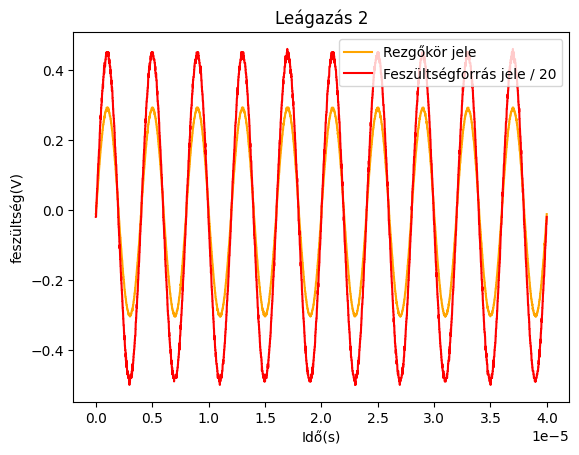
\includegraphics{Leagazas_2.png}
\end{figure}
\begin{figure}[H]
    \centering
    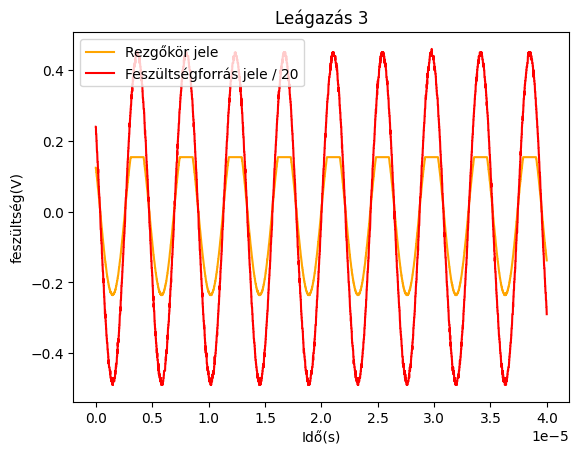
\includegraphics[scale=0.5]{Leagazas_3.png}
\end{figure}
\begin{figure}[H]
    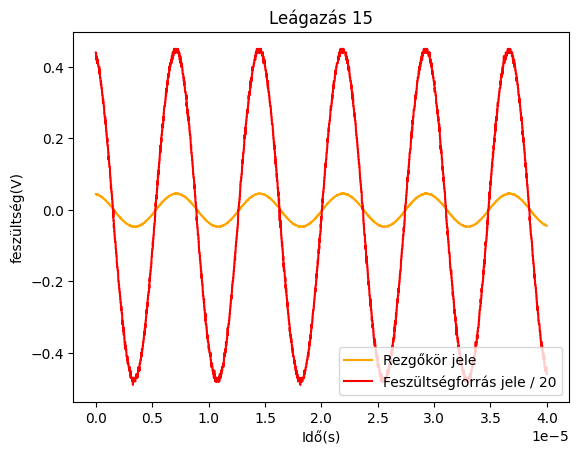
\includegraphics[scale=0.5]{Leagazas_15.png}
    \centering
\end{figure}
A 3. és a 4. leágazáson megfigyelhető volt a 2. ábrán is látható szabálytalanságok a rezgőkör feszültségében, amelyet feltehetően 
az oszciloszkóp hibája okozott.\\ Az így mért adatokra $f_0\left(\ell \right)=\frac{c}{\sqrt{\ell - \beta}}$ alakú függvényt illesztünk, melyben 
$\ell$ az egyetlen változó, $\beta$ a \ref{mckota}-ban is megjelenő $\alpha$ arányossági tényező és $r$ a tekercs sugarának a szorzata.\\ Valamint 
$c=\frac{c_0}{2\pi\sqrt{r^2\pi n^2 \frac{A}{d}}}$.\\Az illesztés paraméterei a hövetkezőknek adódnak:\newline
\begin{centering}
    \begin{tabular}{|r|r|r|}
        \hline
        Paraméter & Érték & Hiba \\
        \hline
        $c$ & $80081,6\frac{m^{1/2}}{s}$ & $25,17\frac{m^{1/2}}{s}$ \\
        \hline
        $\beta$ & $0,0121641\left(m^{1/2}\right)$ & $8,499\cdot 10^{-05}m$ \\
        \hline
    \end{tabular}
\end{centering}
\newline A következő ábrán a mért rezonanciafrekvenciák lesznek láthatóak a hozzájuk tartozó leágazás függvényében:\newline   
\begin{figure}[H]
    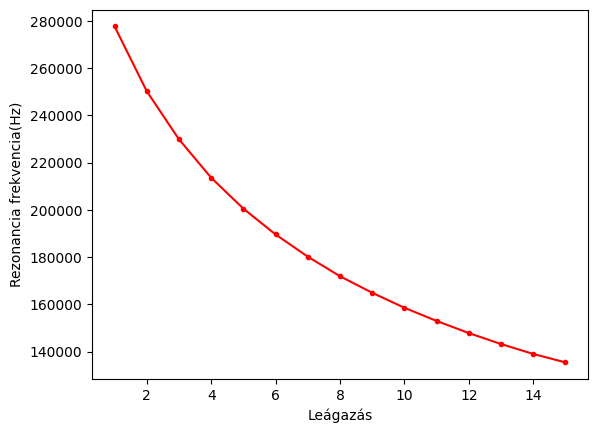
\includegraphics[scale=0.5]{Rezonancia_frekvencia_leagazas.png}
    \centering
\end{figure}
Ezekből $c_0$ és $\alpha$ értékei:
\begin{centering}
    \begin{tabular}{|r|r|r|}
        \hline
        Paraméter & Érték & Hiba \\
        \hline
        $c_0$ & $283655677\frac{m}{s}$ & $5561673\frac{m}{s}$ \\
        \hline
        $\alpha$ & $0,747181$ & $1.0116\cdot 10^{-02}$ \\
        \hline
    \end{tabular}
\end{centering}
\newline
Az alábbiakban a mért rezonanciafrekvenciák, és az illesztett görbe látható a tekercs hosszának függvényében:\newline
\begin{figure}[H]
    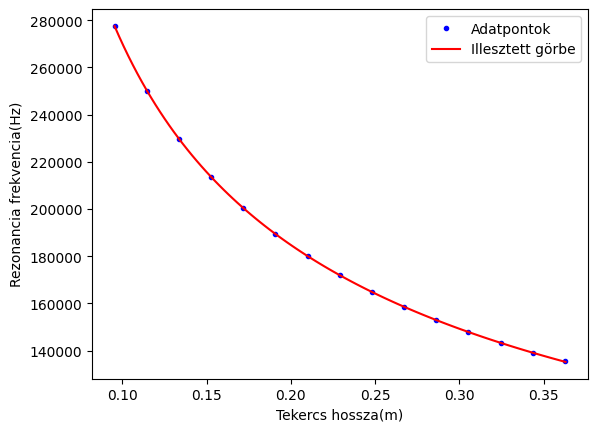
\includegraphics[scale=1]{Rezonancia_frekvencia_hossz.png}
    \centering
\end{figure}
Ahol $c_0$ és $\alpha$ hibáit a következő képletek adják meg:
\begin{eqnarray}
    \delta c_0 &=& \delta c + \frac{2\delta r+2\delta n+\delta A+\delta d}{2} \\
    \delta\alpha &=& \delta\beta + \delta r
\end{eqnarray}
\subsubsection{Rezonanciagörbe vizsgálata}
A 2. leágazáson történt 21 a rezonanciafrekvencia közeli frekvencián történő mérés során kapott amplidúdókra 
Lorentz-görbét illesztünk, melynek az egyenlete a következő:
\begin{equation}
    A\left(f\right)=\frac{M}{\sqrt{\left(f-f_0\right)^2+\frac{B^2}{4}}}
\end{equation}
Ahol $f$ a frekvencia, $f_0$ a rezonanciafrekvencia, $B$ a sávszélesség és $M$ egy arányszám, melynek segítségével figyelembe lehet venni 
a mért feszültség nagyságát.\\Az illesztésből a következő paramétereket kapjuk:
\begin{centering}
    \begin{tabular}{|r|r|r|}
        \hline
        Paraméter & Érték & Hiba \\
        \hline
        $f_0$ & $250589,41Hz$ & $13,3Hz$ \\
        \hline
        $M$ &  $518,0526\frac{V}{s}$ & $3,631\frac{V}{s}$ \\
        \hline
        $B$ & $3494,62Hz$ & $36,293Hz$ \\ 
        \hline
    \end{tabular}
\end{centering}
\newline Az illesztett görbe, és a mért amplitúdók\footnotemark a frekvencia függvényében:\newline
\footnotetext{Az errorbar-ok rosszul látszanak, mivel az amplitúdó hibája kicsi a rezonanciafrekvencia amplitúdójához képest.}
\begin{figure}[H]
    \centering
    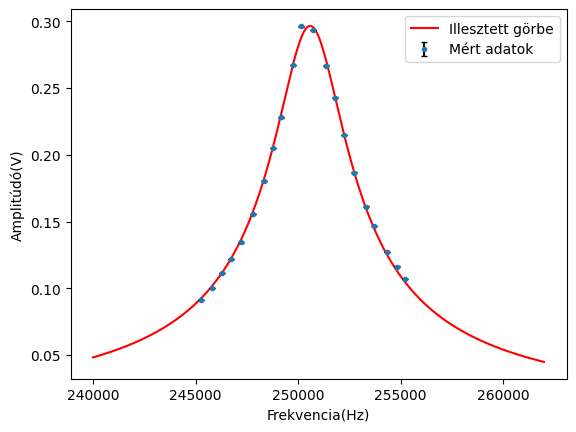
\includegraphics[scale=0.95]{Lorentz_görbe.png}
\end{figure}
Az illesztésből kapott rezonanciafrekvencia nagyjából 300$Hz$-el tér el a mért értéktől, amely azzal magyarázható, hogy mint az ábrán is látható az illesztés 
a rezonanciafrekvencia körüli pontokra pontatlan.\\A szávszélességet vizsgálva is megfigyelhetjük, hogy $f_0\pm B$ pontokban az amplitúdó nem $\frac{1}{\sqrt{2}}$-ed 
része a legnagyobb amplitúdónak, amelyet szintén az illesztés fentebb leírt hibája okozhat.


A kapott sávszélességből, és rezonanciafrekvenciából megkaphatjuk az áramkör jósági tényezőjét, és annak hibáját az alábbi képletekkel:
\begin{eqnarray}
    Q&=&\frac{f_0}{B}\\
    \delta Q &=&\delta f_0 +\delta B
\end{eqnarray}
Amiből $Q=71,0707\pm0,7485$ adódik, ám az illesztett függvény már fentebb tárgyalt problémája miatt ez a valódi értékhez képest valószínűleg hibahatáron kívül lesz.
\section*{Összegzés}
A mérés során kapott adatokból számolt fénysebesség nagyságrandileg megegyezik a valódi értékkel, értéke annál nagyjából $5\%$-al kissebb.
azonban a kapott érték  nincs hibahatáron belül, amely elsősorban az anyagi minőségek elhanyagolásából és a tekercs sugarának méréséből származhat, ugyanis 
utóbbi mivel egy PVC csőre van tekercselve nem egyenletesen kör keresztmetszetű, valamint a keresztmetszete alakja nem állandó a hosszában, hanem kis mértékben változik.
Ezen kívül az eredmény a vasóstól lévő eltérésébe még a tápegység jelének bevezetése, valamint az oszciloszkóp belekötése is beleszólhat.


A rezonanciagörbe vizsgálata során kapott paraméterek pontatlanságába pedig elsősorban a rosszul sikerült függvényillesztés szól bele, azonban itt nem lehet tudni a 
az igazi értékektől való eltérést, hiszen nincsenek referenciaértékek.
%% IRODALOMJEGYZÉK
%\begin{thebibliography}{9}

%\bibitem{lamport94}
%  Leslie Lamport,
%  \textit{\LaTeX: a document preparation system},
%  Addison Wesley, Massachusetts,
%  2nd edition,
%  1994.
%  \url{https://bla.com}

%\end{thebibliography}

\end{document}
